\chapter{Introducción Específica} % Main chapter title

\label{Chapter2}

%----------------------------------------------------------------------------------------
%	SECTION 1
%----------------------------------------------------------------------------------------

Este capítulo provee una introducción más detallada de todo el trabajo realizado.
Se presenta al lector una explicación del funcionamiento  de los semáforos, una vista general del sistema, requerimientos y una explicación de las tecnologías involucradas en el desarrollo.

\section{Funcionamiento de los semaforos}

Los semáforos, también conocidos técnicamente como señales de control de tráfico, son dispositivos de señales que se sitúan en intersecciones viales y otros lugares para regular el tráfico, y por ende, el tránsito peatonal \citep{semaforo}.

Los semáforos se dividen en tres clases, que son: 

\begin{itemize}
\item Vehicular: Tiene por objeto regular el tránsito de vehículos en las intersecciones. Está compuesto esencialmente por tres faros programados para que proyecten durante un tiempo determinado.
\item Peatonal: Se hallan instalados en combinación con los vehiculares y tienen por objeto regular el paso de los peatones en intersecciones con alto volumen de tráfico.
\item Direccional: Tiene como fin informar mediante flechas, el momento adecuado para girar. 
\end{itemize}

En cuanto al funcionamiento del semáforo vehicular se puede decir que, cuando la luz es verde, significa que hay vía libre y se puede pasar. La luz amarilla advierte al conductor que se aproxima un cambio de luz. Al ver la luz roja se debe detener el auto, pues otro flujo de vehículos se interceptará en la dirección de su marcha.

En los semáforos peatonales, el significado es el siguiente: la silueta roja indica que el peatón no debe cruzar la calle, mientras que la silueta verde o blanca lo permite.

En los semáforos direccionales, la flecha roja prohíbe el giro, y la verde autoriza el cruce en ese sentido.

\subsection{Secuencia}
En base a la observación del funcionamiento de los semáforos vehiculares en distintas provincias de la República Argentina como ser Córdoba, Catamarca y Tucumán se detectaron las siguientes secuencias:

\begin{itemize}
\item Rojo, rojo-amarillo , verde, amarillo y rojo
\item Rojo, amarillo, verde, amarillo y rojo
\item Rojo, amarillo, verde y rojo
\end{itemize}

\section{Esquema general del sistema}
Se observa en la siguiente figura \ref{fig:diagramaGeneral} una  version simplificada del sistema.

\begin{figure}[h]
	\centering
	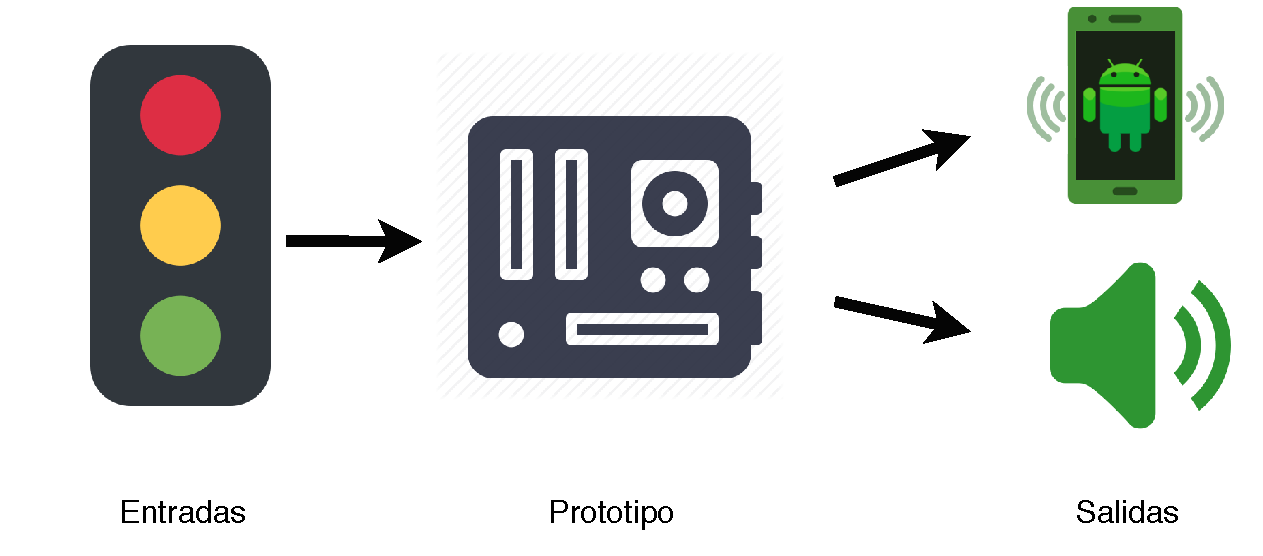
\includegraphics[scale=.6]{./Figures/diagramaGeneral.pdf}
	\caption{Esquema general del sistema.}
	\label{fig:diagramaGeneral}
\end{figure}

Se toman como entradas las luces del semáforo, que se encuentran conectadas al prototipo a través de interfaces que detectan la tensión presente en los focos. Esta información se procesa y según el caso se envían las señales correspondientes. El sistema puede advertir a una persona con discapacidad visual de dos maneras diferentes:

\begin{enumerate}
\item Por medio del módulo Wi-Fi hacia una aplicación instalada previamente en su teléfono inteligente.
\item Mediante una bocina que emite una señal sonora. Para esto el prototipo toma el ruido ambiente y limita la intensidad de esta señal de manera directamente proporcional al ruido presente.
\end{enumerate}

\section{Requerimientos}

De acuerdo a la necesidad que se necesita satisfacer y a lo expuesto, se encontraron los siguientes requerimientos:

\begin{enumerate}[{R}1.]
\item Hardware:
	\begin{enumerate}[{R1.}1.]
		\item Operar con cargas de entradas de 220 V, 50 Hz y 5 A.
		\item El hardware involucrado en la detección del cambio de luces debe estar totalmente aislado del módulo principal.
	\end{enumerate}
\item Comunicación:
	\begin{enumerate}[{R2.}1.]
		\item El sistema debe proveer un red Wi-Fi que cumpla con las normas IEEE 802.11.
		\item Se debe proveer una señal sonora, su intensidad debe poder variar automáticamente dependiendo del ruido presente.
	\end{enumerate}
\item Software embebido:
	\begin{enumerate}[{R3.}1.]
		\item El sistema deberá ser capaz de aprender la secuencia de cambio de luces.
		\item El sistema deberá ser capaz de detectar el semáforo fuera de servicio.
		\item Se deberá implementar un protocolo para la fácil escalabilidad de los distintos tipos de comunicación.
		\item El sistema deberá implementarse en base a un sistema operativo de tiempo real. 
	\end{enumerate}
\item Metodología de desarrollo:
	\begin{enumerate}[{R4.}1.]
		\item Se utilizará GIT como herramienta de control de versiones.
		\item Se utilizará Doxygen como herramienta para generar la documentación.
		\item Se realizarán pruebas unitarias para cada módulo.
	\end{enumerate}
\item Aplicación móvil:
	\begin{enumerate}[{R5.}1.]
		\item Conectarse automáticamente a la red wifi que provee el sistema.
		\item Definir un protocolo de vibraciones según los mensajes del sistema.
	\end{enumerate}
\end{enumerate}

\section{Propuesta de implementación}

Para abordar una solución integral a la problemática planteada y satisfacer los requerimientos enunciados, se propuso un sistema con componentes de hardware y software los cuales se describen de la siguiente manera.

Para el software se utilizaron las siguientes tecnologías:

\begin{itemize}
	\item FreeRTOS como sistema operativo de tiempo real.
	\item sAPI como framework para manejo de periféricos \citep{sapi}.
	\item Colas para mensajes entre tareas.
	\item Eventos asincronicos.
\end{itemize}

En cuanto al hardware, los elementos se dividieron en tres secciones:

\begin{itemize}
	\item Elementos de entrada.
	\item Plataforma de desarrollo.
	\item Elementos de salida.
\end{itemize}

\subsection{Entradas}

\subsubsection{Detección de tension}

Para censar si hay tensión presente en algún foco del semáforo vehicular, se utilizaron módulos de aislamiento con opto-acopladores para corriente
alterna 220 V figura \ref{fig:moduloOptoacoplador} en cada luz. 

\begin{figure}[h]
	\centering
	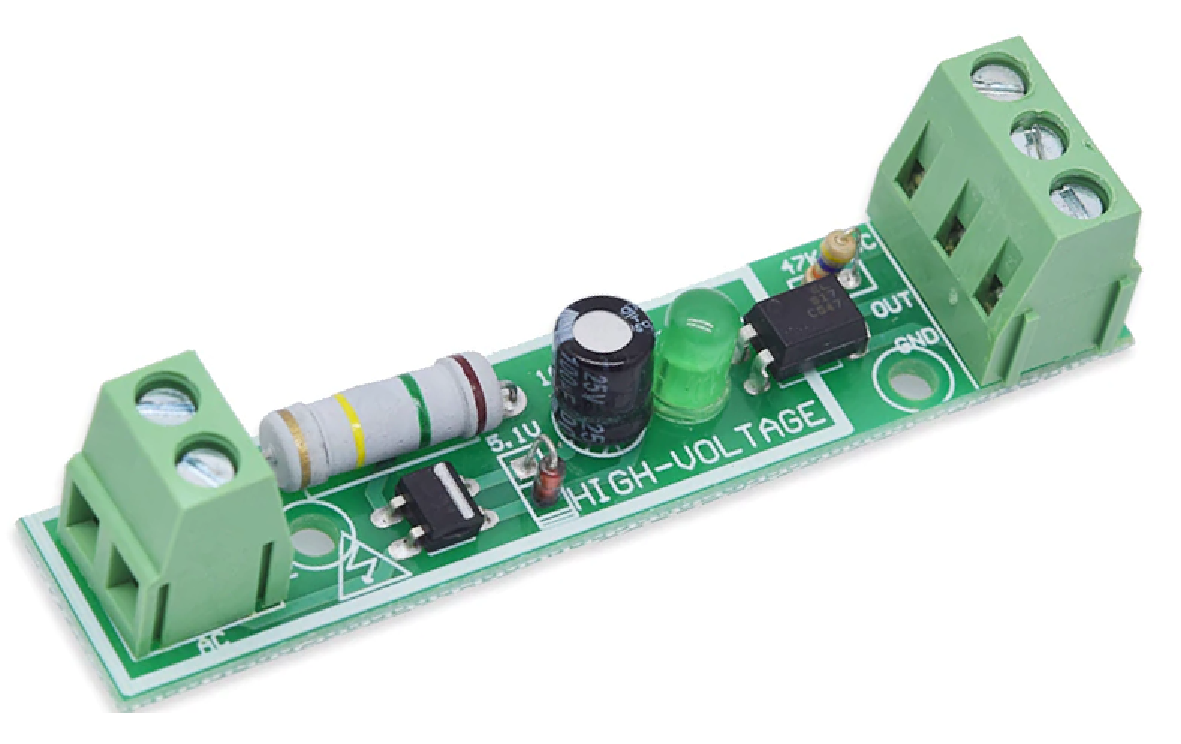
\includegraphics[scale=.3]{./Figures/moduloOptoacoplador.pdf}
	\caption{Módulo de aislamiento opto-acoplador de 1 bit}
	\label{fig:moduloOptoacoplador}
\end{figure}

\subsubsection{Detección de ruido ambiente}

Para la detección del nivel de ruido ambiente presente se utilizo un modulo que tiene un micrófono y un circuito amplificador con un integrado LM393 figura \ref{fig:detectorSonido}.

\begin{figure}[h]
	\centering
	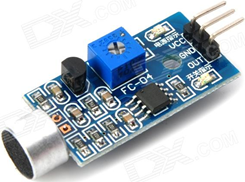
\includegraphics[scale=.5]{./Figures/detectorSonido.png}
	\caption{Módulo para la detección de sonido}
	\label{fig:detectorSonido}
\end{figure}

\subsection{Plataforma de desarrollo}
Se optó por la EDU-CIAA-NXP figura \ref{fig:eduCiaaNxp} como base para el desarrollo del proyecto por ser una plataforma ya conocida, de amplia disponibilidad, económica y de hardware abierto. Dicha placa posee un microcontrolador LPC4337 de la empresa NXP, el cual cuenta con dos núcleos ARM Cortex-M; un Cortex-M4 y un Cortex-M0.

\begin{figure}[H]
	\centering
	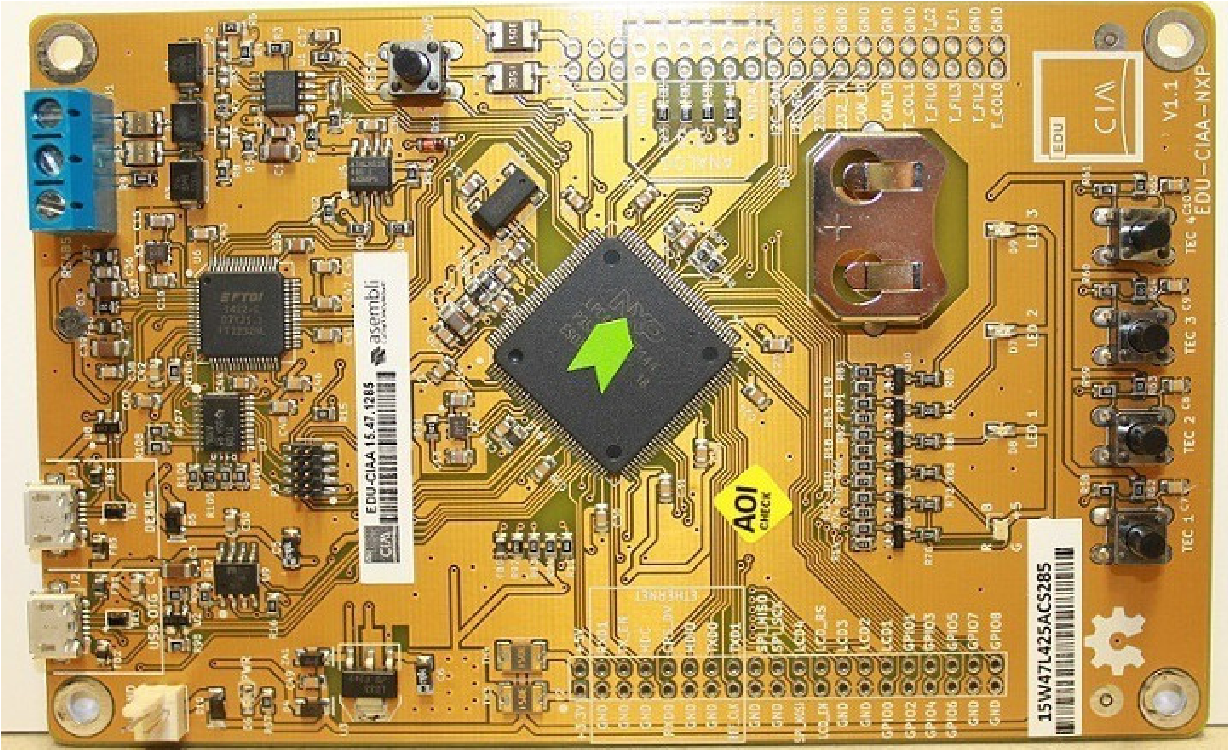
\includegraphics[width=0.7\textwidth]{./Figures/eduCiaaNxp.pdf}
	\caption{La EDU-CIAA posee un microcontrolador LPC4337 (dual core ARM Cortex-M4 y Cortex-M0).}
	\label{fig:eduCiaaNxp}
\end{figure}

\subsection{Salidas}
\subsubsection{Modulo wifi}
El ESP01\citep{esp01} es un modulo que contiene un microcontrolador ESP8266\citep{esp8266} de bajo coste con Wi-Fi integrado fabricado por la empresa Espressif\citep{espressif} figura \ref{fig:esp01}. En cuanto a comunicación Wi-Fi, este modulo tiene comunicación integrada 802.11 b/g/n, incluidos modos Wi-Fi Direct (P2P)\citep{wifiDirect} y softAp\citep{softAp}. Incluye una pila de TCP/IP completa, lo que libera de la mayor parte del trabajo de comunicación al procesador.

\begin{figure}[h]
	\centering
	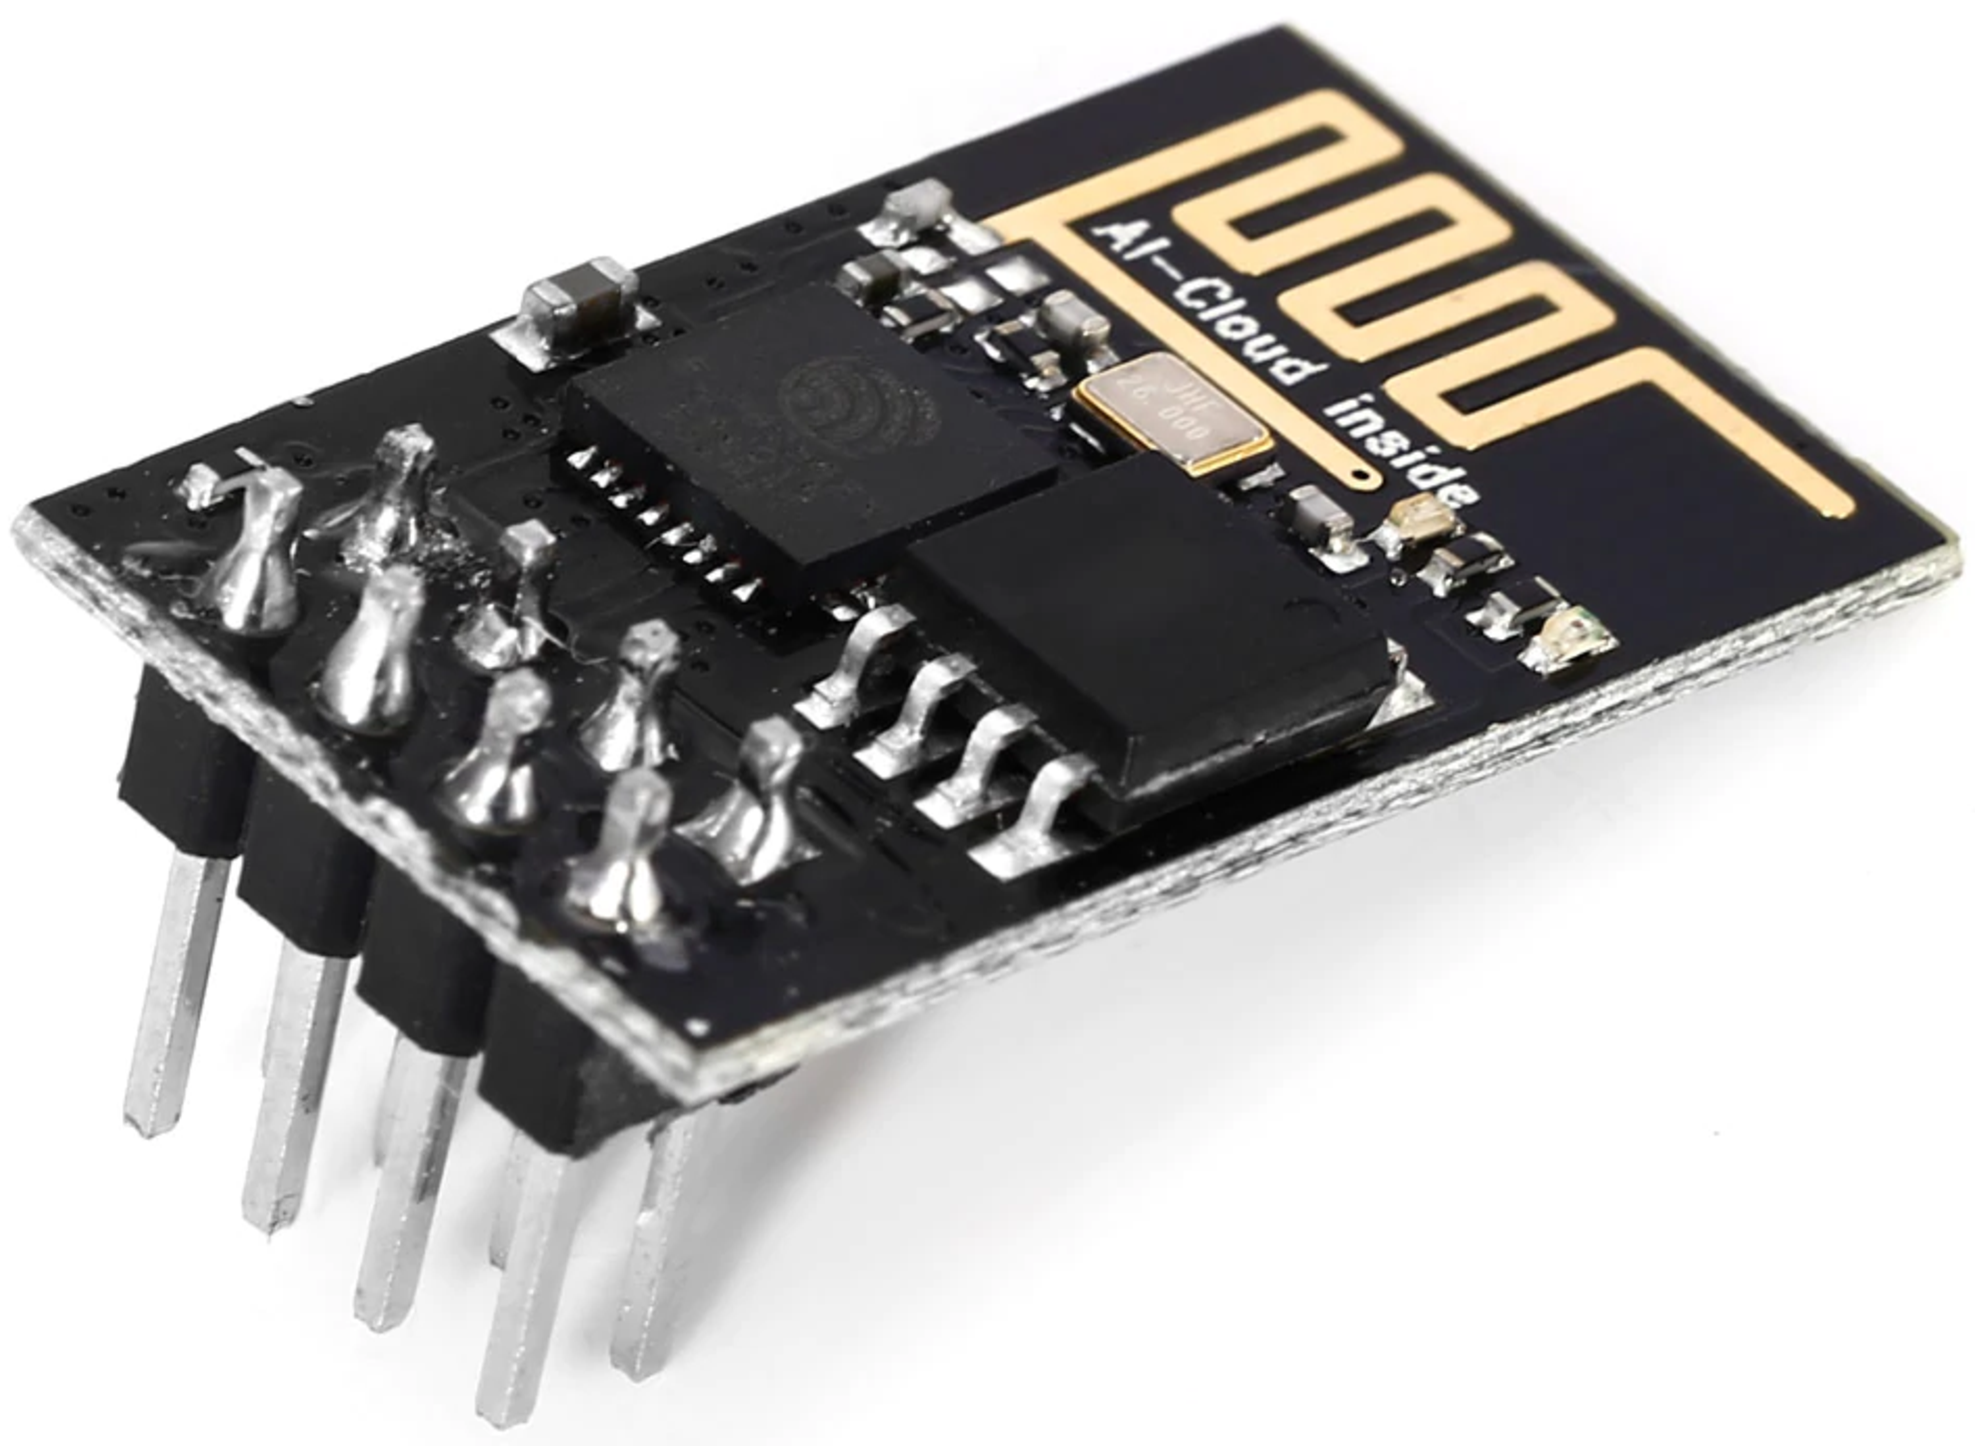
\includegraphics[scale=.2]{./Figures/esp01.pdf}
	\caption{ESP8266 (ESP-01) 2.4GHz Módulo Inalámbrico.}
	\label{fig:esp01}
\end{figure}

\subsubsection{Modulo generador de sonido}
El módulo fue desarrollado específicamente para este proyecto en base a diagramas de la hoja de datos del fabricante figura \ref{fig:amplificadorLM386} para el amplificador operacional LM386\cite{dsLm386}, el cual provee un amplificador de audio de baja potencia, capaz de funcionar con una fuente de alimentación simple entre 4 y 12 V. Este módulo genera una señal sonora a través de un parlante de \SI{8}{\ohm}.

\begin{figure}[h]
	\centering
	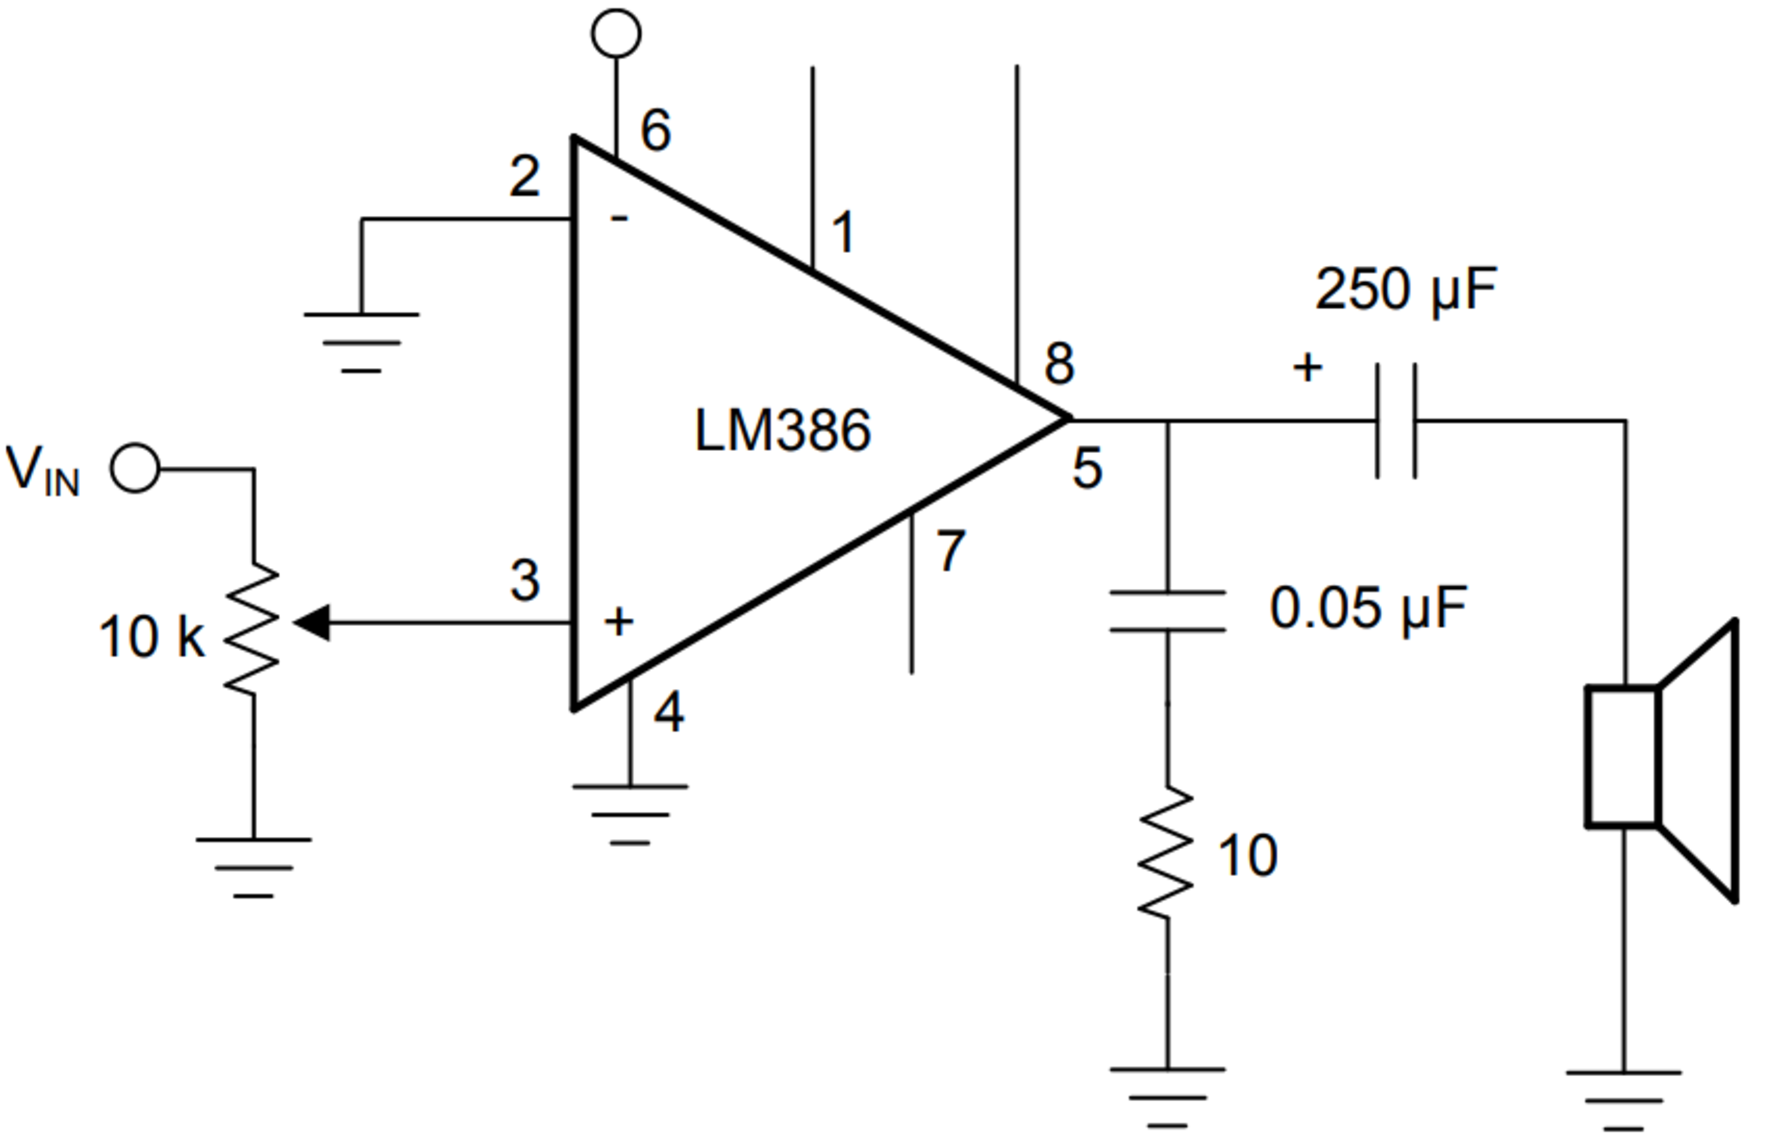
\includegraphics[scale=.35]{./Figures/amplificadorLM386.pdf}
	\caption{Circuito amplificador basado en el amplificador operacional LM386.}
	\label{fig:amplificadorLM386}
\end{figure}
